\documentclass[convert={density=300, outext=.png}, border=0pt]{standalone}

\usepackage[utf8]{inputenc}
\usepackage{tikz}
\usepackage{verbatim}
\usepackage{ulem}

\usetikzlibrary{calc, arrows, positioning}

\begin{document}

	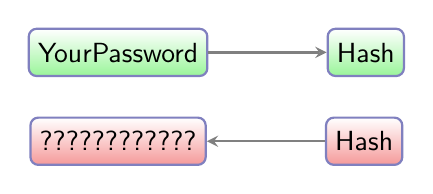
\begin{tikzpicture} [node distance=1.5cm,
		% define styles
		basicnodestyle/.style={
			% The shape:
			rectangle,
			% The size:
			minimum size=6mm,
			% The border:
			thick,
			draw=blue!50!black!50, % 50% blue and 50% black
			% The filling:
			top color=white, % a shadi,ng that is white at the top...
			bottom color=blue!50!black!20, % and something else at the bottom
			% Corners
			rounded corners=1.0mm,
			% Font
			font=\sffamily%\itshape
		},
		deniednodestyle/.style={
			% The shape:
			rectangle,
			% The size:
			minimum size=6mm,
			% The border:
			thick,
			draw=blue!50!black!50, % 50% blue and 50% black
			% The filling:
			top color=white, % a shadi,ng that is white at the top...
			bottom color=red!90!black!40, % and something else at the bottom
			% Corners
			rounded corners=1.0mm,
			% Font
			font=\sffamily%\itshape
		},
		grantednodestyle/.style={
			% The shape:
			rectangle,
			% The size:
			minimum size=6mm,
			% The border:
			thick,
			draw=blue!50!black!50, % 50% blue and 50% black
			% The filling:
			top color=white, % a shadi,ng that is white at the top...
			bottom color=green!90!black!40, % and something else at the bottom
			% Corners
			rounded corners=1.0mm,
			% Font
			font=\sffamily
		},
		arrow/.style={
			->,
			% Thickness
			thick,
			>=stealth,
			% Color
			black!50,
			text=black,
			font=\small
		},
		arrowresponse/.style={
			->,
			% Thickness
			thick,
			>=stealth,
			% Color
			black!50,
			text=black!90,
			font=\small
		}]
		% end of style definition
		
		% draw nodes
		\node (iPassword) [grantednodestyle] {YourPassword};
		\node (iHashing1) [grantednodestyle, right = of iPassword] {Hash};

		\node (iUnknown) [deniednodestyle, below= of iPassword, yshift=1.0cm] {????????????};
		\node (iHashing2) [deniednodestyle, right = of iUnknown] {Hash};
		
		% connect nodes
		\draw [arrow] (iPassword) -- (iHashing1);
		\draw [arrow] (iHashing2) -- (iUnknown);
	\end{tikzpicture}
	
\end{document}

% use pdflatex -shell-escape password_certification_creation.tex to compile this into png
